\chapter{Conclusion}
We have developed a web-based proof assistant which lets users define syntax and inference rules in \LaTeX{} and verifies derivations built in the web interface against the user-defined rules. To support these functionalities, we have devised algorithms for parsing syntax rules, inference rules, and user-inputted terms, as well as verifying derivations by matching names to ASTs. \Cref{fig:conclusion:flowchart} summarises the roles of the various algorithms in this project.

\begin{figure}[!htbp]
    \centering
    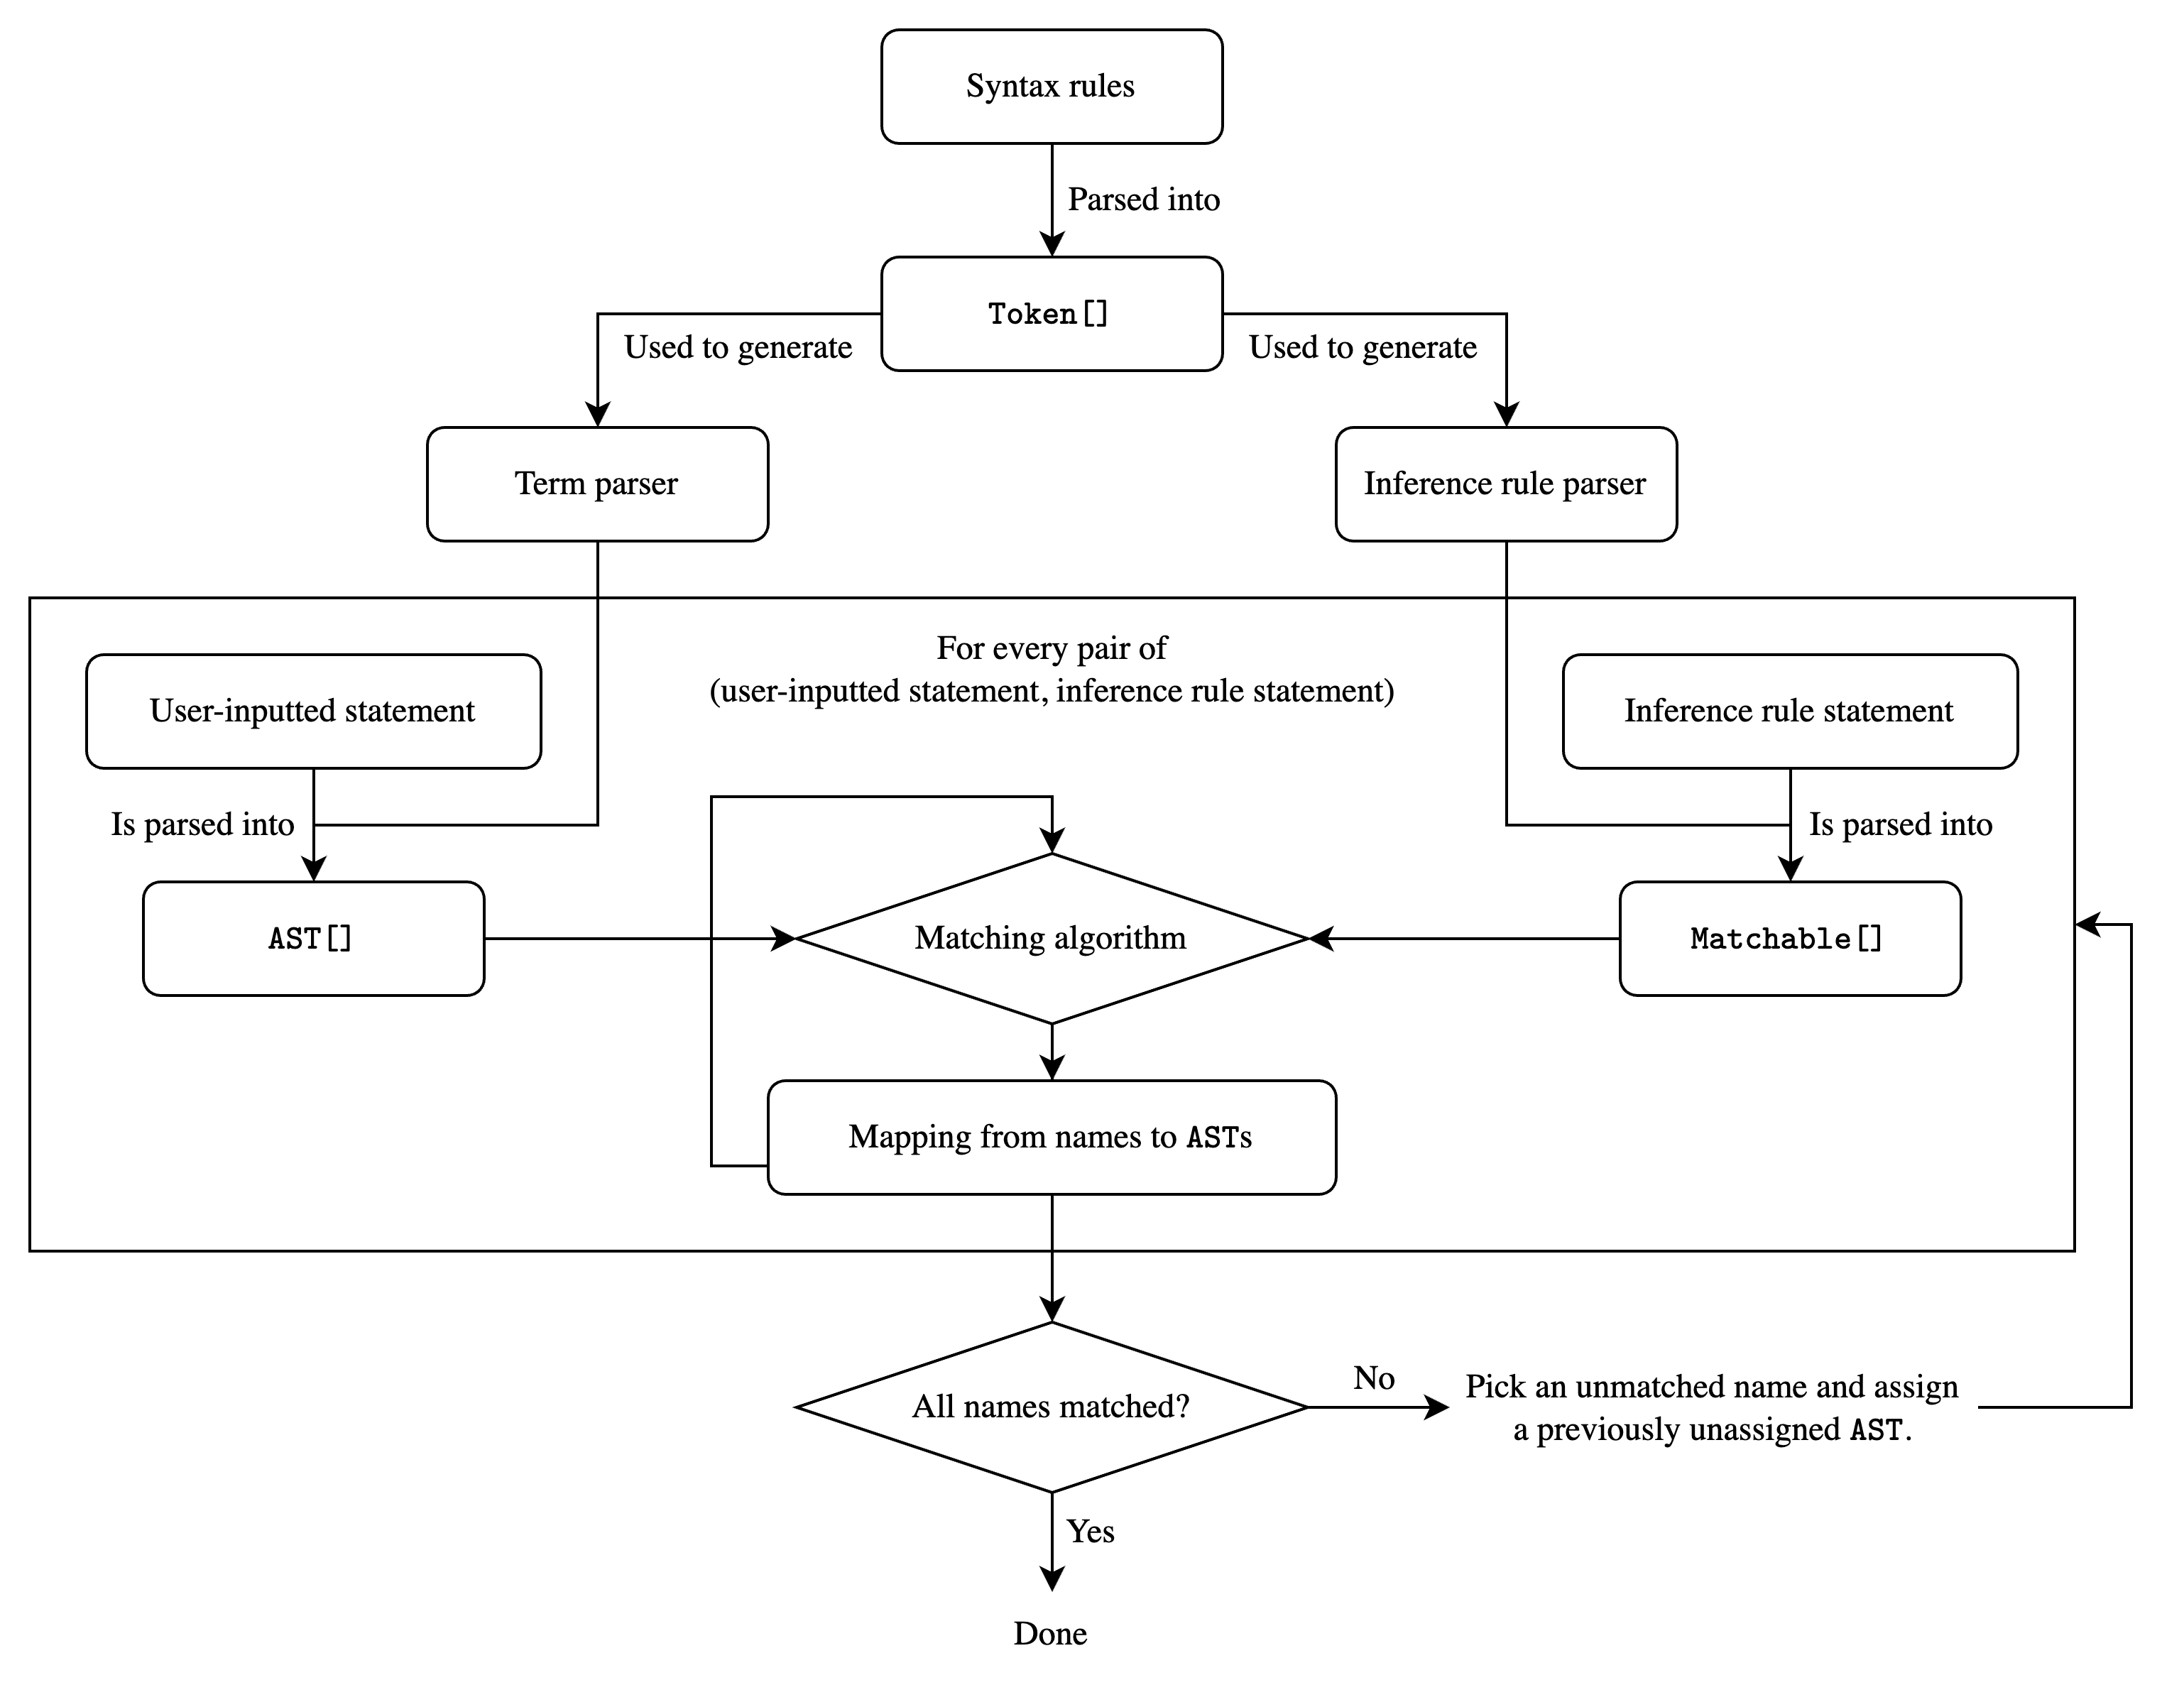
\includegraphics[width=\textwidth]{conclusion/flowchart.png}
    \caption{A flowchart showing the process of verifying whether an inference rule is applied correctly}
    \label{fig:conclusion:flowchart}
\end{figure}

The algorithms were evaluated and refined by testing against example derivations in natural deduction, the simply typed $\lambda$-calculus, the system \textsc{lk}, the $\lambda$-calculus with pairs and product types, and the calculus \lbm. The user experience of the application was evaluated and refined by asking users to build derivations and observing their behaviour.

\section{Future work}
\subsection{Bracketing conventions and abbreviations}
One of the biggest limitations preventing the current web application from becoming a fully ergonomic and intuitive extension of writing derivations by hand is its inability to parse abbreviated terms, including terms that are not fully bracketed.

When writing derivations by hand, we often drop the outermost parentheses and any parentheses that are implied by associativity conventions. For example, the Curry type $(1 \to (2 \to 3))$ is usually abbreviated as $1 \to 2 \to 3$, since $\to$ is right-associative. One solution may be to treat parentheses as special characters and let the user specify operator associativity whenever the definition contains a pair of parentheses. However, it is difficult to determine the operator within the input enclosed by the parentheses. Suppose the user adds symbols to the definition of Curry types:
\[
    A, B \Coloneqq \varphi \alt (A* \to{} +B)
\]
Unless the application treats $\to$ differently from $*$ and $+$, all three symbols are equally likely to be the principal connective in this case. Therefore, the application must either define a set of special symbols as operators or allow the user to specify the operator.

A better solution is to let the user define rewriting rules that capture both associativity and the convention of dropping the outermost parentheses. In the case of Curry types, the user might specify
\begin{align*}
    (A \to (B \to C)) \quad &\to \quad A \to B \to C \\
    (A \to B) \quad &\to \quad A \to B
\end{align*}
where the $\to$ in the middle means ``can be abbreviated as''. One way to preprocess the input according to the re-writing rules is as follows:
\begin{enumerate}
    \item Generate parsers for each of the abbreviations, i.e. the terms on the right of the $\to$.
    \item Apply the abbreviation parsers from top to bottom and stop as soon as a parser succeeds.
    \item Replace the abbreviation with the fully parenthesised form as specified on the left of the $\to$.
    \item Repeat steps 2 to 3 until no more re-writing rules can be applied.
    \item Proceed to the next part of the input.
    \item Repeat steps 2 to 5 until all input is consumed.
\end{enumerate}
Once the input is fully preprocessed, it should be fully parenthesised and ready to be parsed in the manner described in the previous chapters. If the preprocessing algorithm is properly implemented, it should be able to accept both inference rule statements and user-inputted terms as input.

One issue with this solution is that preprocessing from left to right does not always produce the correct result. Consider the abbreviated term $1 \to 2 \to 3 \to 4$. When applied to this term, the preprocessing algorithm described above proceeds as follows:
\begin{enumerate}
    \item Apply the first re-writing rule to get $(1 \to (2 \to 3)) \to 4$.
    \item Apply the second re-writing rule to get $((1 \to (2 \to 3)) \to 4)$.
    \item Neither of the re-writing rules can be applied, so the algorithm terminates.
\end{enumerate}
However, the output should have been $(1 \to (2 \to (3 \to 4)))$ instead. The preprocessing algorithm would have obtained the correct output if it were applied from right to left, since the first step of the algorithm would have returned $1 \to (2 \to (3 \to 4))$.

One way around this issue is to define a special symbol $\cdots$ meaning ``and so on''. The re-writing rules above can be simplified as the rule
\[
    (A_1 \to (A_2 \to \cdots (A_{n-1} \to A_n))) \quad \to \quad A_1 \to A_2 \to \cdots \to A_n
\]
But then the main difficulty becomes interpreting $\cdots$ correctly. Another way around this issue is to enumerate the re-writing rules up to a certain point and not handling any abbreviations beyond that point. For example, the user may choose to only handle abbreviations for Curry types with up to four arrows:
\begin{align*}
    (A \to (B \to (C \to (D \to E)))) \quad &\to \quad A \to B \to C \to D \to E \\
    (A \to (B \to (C \to D))) \quad &\to \quad A \to B \to C \to D \\
    (A \to (B \to C)) \quad &\to \quad A \to B \to C \\
    (A \to B) \quad &\to \quad A \to B
\end{align*}
The latter workaround also works for abbreviations of abstractions in the $\lambda$-calculus, too. In general, the abstraction $(\lambda x_1. (\lambda x_2. \cdots (\lambda x_n. M)))$ can be abbreviated as $\lambda x_1 x_2 \cdots x_n. M$. Ideally, the abbreviation can be expressed by the following re-writing rule:
\[
     (\lambda var_1. (\lambda var_2. \cdots (\lambda var_n. M))) \quad \to \quad \lambda var_1 var_2 \cdots var_n. M
\]
But the same difficulty of interpreting $\cdots$ remains. Instead, enumerating abbreviations up to a certain number of variables would work well:
\begin{align*}
    (\lambda var_1. (\lambda var_2. (\lambda var_3. (\lambda var_4. (\lambda var_5. M))))) \quad &\to \quad \lambda var_1\ var_2\ var_3\ var_4\ var_5. M \\
    &\vdotswithin{\to} \\
    (\lambda var_1. M) \quad &\to \quad \lambda var_1. M
\end{align*}

\subsection{Using and proving lemmas}
Suppose a user wants to prove the following conclusion in the system \textsc{lk}:
\begin{equation}
    \varnothing \vdash (((x \to y) \to x) \to x) \land (((y \to z) \to y) \to y)
    \label{eqn:conclusion:peirce}
\end{equation}
The user can build the derivation as follows:
\[
    \Inf[\land R]{
        \textcolor{ForestGreen}{\Inf[\arr R]{
            \Inf[CR]{
                \Inf[\arr L]{
                    \Inf[\arr R]{
                        \Inf[Ax]{x \vdash y, x}
                    }{\varnothing \vdash (x \to y), x}
                    \quad
                    \Inf[Ax]{x \vdash x}
                }{(x \to y) \to x \vdash x, x}
            }{(x \to y) \to x \vdash x}
        }{\varnothing \vdash ((x \to y) \to x) \to x}}
        \quad
        \textcolor{blue}{\Inf[\arr R]{
            \Inf[CR]{
                \Inf[\arr L]{
                    \Inf[\arr R]{
                        \Inf[Ax]{y \vdash z, y}
                    }{\varnothing \vdash (y \to z), y}
                    \quad
                    \Inf[Ax]{y \vdash y}
                }{(y \to z) \to y \vdash y, y}
            }{(y \to z) \to y \vdash y}
        }{\varnothing \vdash ((y \to z) \to y) \to y}}
    }{\varnothing \vdash (((x \to y) \to x) \to x) \land (((y \to z) \to y) \to y)}
\]
Notice the \textcolor{ForestGreen}{green} and \textcolor{blue}{blue} sub-derivations are identical modulo renaming. It would be convenient to be able to turn the sub-derivation into a lemma, prove the lemma, and be able to use the lemma in another derivation. In this example, the lemma
{
    \derivationfont
    \[
        (\textsf{Peirce}): \frac{}{\varnothing \vdash ((var_1 \to var_2) \to var_1) \to var_1}
    \]
}%
would be proven as follows:
\[
    \Inf[CR]{
        \Inf[\arr L]{
            \Inf[\arr R]{
                \Inf[Ax]{var_1 \vdash var_2, var_1}
            }{\varnothing \vdash (var_1 \to var_2), var_1}
            \quad
            \Inf[Ax]{var_1 \vdash var_1}
        }{(var_1 \to var_2) \to var_1 \vdash var_1, var_1}
    }{(var_1 \to var_2) \to var_1 \vdash var_1}
\]
The derivation for \ref{eqn:conclusion:peirce} could be simplified to
\[
    \Inf[\land R]{
        {\Inf[\textsf{Peirce}]{\varnothing \vdash ((x \to y) \to x) \to x}}
        \quad
        \Inf[\textsf{Peirce}]{\varnothing \vdash ((y \to z) \to y) \to y}
    }{\varnothing \vdash (((x \to y) \to x) \to x) \land (((y \to z) \to y) \to y)}
\]
Most of the work needed to support the use of lemmas is in extending the user interface. It would need to track lemmas and their proofs, since it currently only supports one derivation at a time. The algorithms and data structures can handle most backend tasks associated with the use of lemmas, since a lemma is essentially an inference rule associated with a proof, and the algorithms can handle both custom inference rules and verifying proofs. The only task left is to link the lemma with its proof, which can be done in one of two ways:
\begin{itemize}
    \item Construct the proof using placeholders (e.g. $var_1$ and $var_2$ instead of $x$ and $y$). Since placeholders are forbidden from user-inputted terms, a new parser is needed for parsing user-inputted terms and statements in lemma proofs. One way is to parse placeholders as strings and transform them into \lstinline{TerminalAST}s.
    \item Construct the proof using user-inputted statements compatible with the structures of the statements in the lemma. For example, the lemma $(\textsf{Peirce})$ above may be proved by deriving the conclusion $\varnothing \vdash ((x \to y) \to x) \to x$ instead of $\varnothing \vdash ((var_1 \to var_2) \to var_1) \to var_1$. Matching user-inputted statements with the structure of a lemma requires more stringent checks than matching user-inputted statements with the structure of an inference rule when verifying proofs. For example, deriving the conclusion $\varnothing \vdash x \lor (\lnot x)$ does not prove the lemma
    \[
        (\textsf{LEM?}): \frac{}{\varnothing \vdash A \lor B}
    \]
    even though the conclusion is considered compatible with the structure of the conclusion when verifying proofs, since $A$ maps to $x$ and $B$ maps to $(\lnot x)$.
\end{itemize}
% A necessary additional check is to ensure distinct placeholders correspond to distinct user-inputted terms.